% Chapter Template

\chapter{Simulation Environment} % Main chapter title

\label{Chapter 1} % Change X to a consecutive number; for referencing this chapter elsewhere, use \ref{ChapterX}

\lhead{Chapter 1. \emph{Simulation Environment}} % Change X to a consecutive number; this is for the header on each page - perhaps a shortened title

%----------------------------------------------------------------------------------------
%	SECTION 1
%----------------------------------------------------------------------------------------
The first task of my project was to build a simulator to be able to get feedback from a simulated world. The goal of the simulator is to provide an environment which is governed by physics laws. In this project such physics laws are gravity, friction and collisisons. Combining this two phenomena on complex structure can lead to situations difficult to predict, especially since it has a chaotic behavior. Two movements of a structure in such a physical world, though they differ just a little, can lead to very different outcomes.  

\section{Physics Engine}

In order to simulate the behavior of complex shapes and bodies in a simulated world, a physical engine is required. This kind of physical engine is used in a lot of different areas, for instance the film and video games industry, to simulate destructions or complex situations where placing all bodies by hand would be too difficult. I tested two different librairies that provide tools to simulate these complex situtations : \verb?bullet? \verb?ODE? (\verb?Open Dynamics Engine?). The first part was to simulate the static part of the world, which is the ground. For now, I used a plane, with a friction coefficient, but we can imagine testing all the structure on different surfaces, (not necessarly plans). Also in order to simplify the structure, so that the modules are simple shapes, all the robots are only composed of cubes, linked by different type of joints. ODE and bullet also provide tools to simulate joints (adding constraint on the relative movements of different bodies) and also to animate them simulating motors. I choose ODE for its simplicity to control different joints using this motors. In order to simulate a servomotor properly, it is for instance possible to set a maximimum torque value and a command to the motor.

\begin{figure}[htbp]
    \centering
    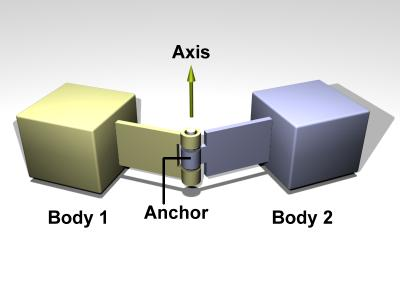
\includegraphics{Figures/hinge.jpg}
    \rule{35em}{0.5pt}
    \caption[A Hinge Constraint]{A 3D representation of a Hinge Constrain}
    \label{fig:Hinge}
\end{figure}

\section{Visual rendering}
A good thing about the physical engine is that it is completly separated from the rendering part. That way, it is possible to run much faster for the learning process. But it is also necessary to see the result, especially for the purpose of debuging the simulator. Carnegie Mellon University developps a framework called panda3d, that integrate both a rendering librairy using OpenGl and different physics engines (ODE and bullet). All this tools are developped in C/C++ with binding for python, which makes it an easy tool to create animation movie, games or simulations.

\subsection{The coordinate system}
In order to represent all the objects that we manipulate in the simulation (physics and rendering), panda3d uses a system of global/local coordinate and a tree architecture. Each element of the tree is represented in the coordinates of the father. In order to keep a coherence with this architecture, it is natural to use a graph to represent the modular structure of the robots. Panda3d also uses 4-by-4 matrices to represent the transformation of a node to its one of its children. These transformation are classical in 3d representation. They combine the benefits of 3 by 3 matrices that represent functions ($\mathbb{R}^3 \to \mathbb{R}^3$) that can be interpreted as the set of combined rotations and homotetia, where the matrix multiplication is the composition of such transformations, and a translation. Manipulating translations requires to use 4 by 4 matrices instead of 3 by 3 but the properties of the product are kept, which makes it a very useful tool to manipulate 3d objects. For instance, if the children of the node is translated of a vector $(1, 0, 0)$, then we can use a function on the object representing the Matrice (TransformState in panda3d) to change the matrice and add the translation. The same goes for giving a certain orientation to the object using quaternions to represent the 3D orientation and add this to the 4 by 4 matrix.

## Picture of the 4*4 Matrix ##

\section{Structures of the Robots as a Graph} 

We can represent a Robot as a graph, where each node is a component of the robot. In this project there is four types of components : 
\begin{itemize}
    \item the head: which has a cube shapes and 6 sons (one for each faces), There is only one head per structure.
    \item a structural block: This is also a cube, also with 6 sons (or edges in the graph) for all faces.
    \item a hinge joint: The hinge is composed of two small cubes, separated by the joint whith one degree of freedom.
    \item a vertebra : a vertebra is very much like a hinge but has two degrees of freedom (two angle directions) with smaller range, but bigger maximal torque.
\end{itemize}

## Picture of Hinge and vertebra ? ##

This Structure is represented in python with an object called MetaStructure, with very simple function to move within the graph and add components and follow edges that make it easy to design a structure that we have in mind, ( or for possible later use to generate them automaticly\ldots). This object is the key to describe a structure.  
    
